\clearpage
\setmonofont[Mapping=tex-text]{CMU Typewriter Text}
\section{Обзор}
Алгоритм, доработке которого посвящена данная работа, основан на алгоритме RNGLR~\cite{RNGLR} (Right-Nulled Generalized LR). В свою очередь, RNGLR является модификацией алгоритма Generalized LR (GLR)~\cite{Tomita}, предназначенного для анализа естественных языков. GLR-алгоритм использует управляющие таблицы семейства LR (Left-to-right Rightmost) алгоритмов~\cite{Grune} с возможностью содержать несколько действий в одной ячейке. Таким образом, при описании работы алгоритма ослабленного синтаксического анализа регулярной аппроксимации динамически формируемого выражения необходимо рассмотреть все вышеперечисленные алгоритмы.

В данном разделе дано краткое описание работы алгоритма ослабленного синтаксического анализа регулярной аппроксимации динамически формируемого выражения. Также рассмотрено понятие синтаксической ошибки в алгоритмах LR-семейства и описан проект, в рамках которого велась разработка предложенного алгоритма.

\subsection{Регулярная аппроксимация динамически формируемого выражения}
Под регулярной аппроксимацией подразумевается аппроксимирование сверху множества значений динамически формируемого выражения некоторым регулярным выражением. В терминах привычных для задач распознавания, проверка корректности выражений из аппроксимирующего множества формулируется как задача проверки включения регулярного языка в другой (как правило, контекстно-свободный язык), которая разрешима во многих важных на практике случаях~\cite{LangInclusion}. Метод построения рассматриваемой аппроксимации, представленный в работе~\cite{RegOverApprox}, реализован~\cite{YCregapprox} в проекте YaccConstructor.

\subsection{Алгоритм ослабленного синтаксического анализа регулярной аппроксимации динамически формируемого выражения}
Чтобы понять принцип работы данного алгоритма, сначала рассмотрим алгоритмы LR-семейства, такие как LR(1), SLR(1), LALR(1). Все эти алгоритмы принимают на вход строку и контекстно-свободную грамматику. Если удалось построить детерминированную управляющую таблицу по данной грамматике, то перечисленные алгоритмы позволяют ответить на вопрос о принадлежности произвольной строки языку, порождаемому данной грамматикой. Входная строка читается слева направо и в процессе чтения программа, выполняющая синтаксический анализ, (\emph{парсер}) меняет свои состояния по правилам, установленным в управляющей таблице. Нужная ячейка таблицы определяется текущим состоянием и правым контекстом (одним или несколькими следующими терминалами) входной строки. История состояний программы хранится в виде стека. Кроме перехода из состояния в состояние ячейка управляющей таблицы содержит действия, которые бывают двух видов: \emph{сдвиг} (\emph{push, shift}) --- чтение следующей части входной строки и \emph{свертка} (\emph{reduce}) --- применение одного из правил входной грамматики. Строка принимается алгоритмом лишь в том случае, если она была полностью обработана, и конечное состояние парсера --- одно из заранее определенных \emph{принимающих состояний}.

Иногда построить детерминированную таблицу не удается, и в одной ячейке управляющей таблицы могут быть конфликты следующих видов: сдвиг/свертка (shift/ reduce) и свертка/свертка (reduce/reduce). Существует два подхода, применяемых к обработке таких неоднозначностей. Первый из них подразумевает разрешение конфликтов, а второй --- анализ всех возможных последовательностей действий, предпринимаемых парсером. Алгоритмы семейства GLR, разработанные для анализа произвольных неоднозначных контекстно-свободных грамматик, используют второй подход. При работе этих алгоритмов порождается множество стеков состояний и деревьев разбора, для эффективного хранения которых используются специализированные структуры данных: структурированный в виде графа стек GSS (Graph Structured Stack) и компактное представление леса разбора SPPF~\cite{SPPF} (Shared Packed Parse Forest).

Следует отметить, что оригинальный GLR-алгоритм не способен анализировать все контекстно-свободные грамматики, поэтому в работе~\cite{RNGLR} был предложен RNGLR-алгоритм, который является его расширением. RNGLR специальным способом обрабатывает \emph{обнуляемые справа правила} входной грамматики (имеющие вид $\mathrm{A} \rightarrow \alpha \beta$, где $\beta$ выводит пустую строку $\epsilon$). RNGLR, как и GLR, строит GSS "слоями", т.е. сначала выполняются все возможные операции свертки для текущего терминала, после чего осуществляется операция сдвига к следующему терминалу входной строки. Вершина GSS представляется в виде пары $(s,l)$, где $s$~--- состояние парсера, а $l$~--- уровень (позиция текущего терминала во входном потоке).

Алгоритм, доработке которого посвящена данная работа, является расширением алгоритма RNGLR, способным производить синтаксический анализ регулярного множества входных строк. При анализе рассматриваемым алгоритмом регулярного множества, состоящего из единственной строки конечной длины, результат будет аналогичен результату анализа алгоритма RNGLR. В расширении вместо строки на вход подается конечный недетерминированный автомат с единственными начальным и конечным состояниями, который порождает регулярную аппроксимацию значений динамически формируемого выражения. Данный автомат представляется в виде ориентированного графа (далее \emph{входного графа}) с вершинами --- состояниями автомата и ребрами --- переходами автомата. Строится \emph{внутренний граф}, который получается из входного --- ассоциацией вершин GSS и некоторых коллекций с вершинами графа. Основная идея расширения заключается в перемещении по внутреннему графу и последовательном построении GSS. В качестве "слоев" выступают вершины внутреннего графа, таким образом каждая вершина GSS хранит состояние парсера $state$ и уровень $level$ (который отождествляется с вершиной внутреннего графа). Теперь операция сдвига выполняется не по одному токену, а по множеству токенов, нагруженных на дуги, исходящие из текущей вершины графа.

Для организации порядка обработки вершин внутреннего графа используется глобальная очередь $Q$. При добавлении новой вершины GSS сначала все \emph{свертки длины 0} (\emph{zero-reductions}) добавляются в очередь операций reduce, после этого выполняется операция сдвига следующих токенов со входа, а соответствующие вершины графа добавляются в очередь $Q$. Так как добавление нового ребра GSS может порождать новые свeртки, то в очередь на обработку $Q$ необходимо добавить вершину внутреннего графа, которой соответствует начальная вершина добавленного ребра (процесс построения GSS описан в алгоритме~\ref{gss_construction}). Операции свертки проводятся вдоль путей в GSS, таким образом, если начальная вершина нового ребра ранее присутствовала в GSS, то необходимо заново вычислить свертки путей, проходящих через эту вершину (функция applyPassingReductions в алгоритме~\ref{processVertex}).

Кроме состояния анализатора $state$ и уровня $level$, в вершине GSS хранится коллекция \emph{проходящих сверток}. Проходящая свертка~--- это тройка $(startV, N, l)$, соответствующая свертке, чей путь содержит данную вершину GSS, а длина оставшейся части пути равна $l$. Проходящие свeртки сохраняются в каждой вершине пути (кроме первой и последней) во время поиска путей в функции $makeReductions$ (алгоритм~\ref{processVertex}).
% * <Екатерина Вербицкая> 17:13:17 12 May 2016 UTC+0300:
% А на кой они нужны?

В вершинах внутреннего графа хранятся следующие коллекции:
% * <Екатерина Вербицкая> 17:34:27 12 May 2016 UTC+0300:
% Зачем?
\begin{itemize}
  \item \emph{processed} --- вершины GSS, для которых ранее были вычислены все операции push;
  \item \emph{unprocessed} --- вершины GSS, операции push для которых ещё только предстоит выполнить;
  \item \emph{reductions} --- очередь операций reduce, которые ещё только предстоит выполнить;
  \item \emph{passingReductionsToHandle} --- пары из вершины GSS и ребра GSS, вдоль которых необходимо обновить проходящие свeртки.
\end{itemize}


% * <Екатерина Вербицкая> 18:13:02 12 May 2016 UTC+0300:
% Эти алгоритмы надо как-нибудь вписать. Хотя бы сказать, что если хочется узнать больше -- стоит почитать листинги.
\begin{algorithm}[H]
\begin{algorithmic}[1]
\caption{Алгоритм ослабленного синтаксического анализа регулярной аппроксимации динамически формируемого выражения}
\label{parsing}
\Function{parse}{$grammar, automaton$}
  \State{$inputGraph \gets$ construct inner graph representation of $automaton$}
  \State{$parserSource \gets$ generate RNGLR parse tables for $grammar$}
  \If{$inputGraph$ contains no edges}
    \If{$parserSource$ accepts empty input} {report success}
    \Else { report failure}
    \EndIf
  \Else
    \State{\Call{addVertex}{$inputGraph.startVertex, startState$}}
    \State{$\mathcal{Q}.Enqueue(inputGraph.startVertex)$}
    \While{$Q$ is not empty}
      \State{$v \gets \mathcal{Q}.Dequeue()$}
      \State{\Call{makeReductions}{$v$}}
      \State{\Call{push}{$v$}}
      \State{\Call{applyPassingReductions}{$v$}}
    \EndWhile
    \If{$\exists v_f: v_f.level = q_f$ and $v_f.state$ is accepting} {report success}
    \Else { report failure}
    \EndIf
  \EndIf
\EndFunction
\end{algorithmic}
\end{algorithm}

\clearpage
\begin{algorithm}[H]
\begin{algorithmic}[1]
\caption{Обработка вершины внутреннего графа}
\label{processVertex}
\Function{push}{$innerGraphV$}
  \State{$\mathcal{U} \gets$ copy $innerGraphV.unprocessed$}
  \State{clear $innerGraphV.unprocessed$}
  \ForAll{$v_{h}$ in $\mathcal{U}$}  
    \ForAll{$e$ in outgoing edges of $innerGraphV$}
      \State{$push \gets$ calculate next state by $v_{h}.state$ and the token on $e$}
      \State{\Call{addEdge}{$v_{h}, e.Head, push, false$}}
      \State{add $v_{h}$ in $innerGraphV.processed$}
    \EndFor
  \EndFor
\EndFunction

\Function{makeReductions}{$innerGraphV$}
  \While{$innerGraphV.reductions$ is not empty}
    \State{$(startV, N, l) \gets innerGraphV.reductions.Dequeue()$}
    \State{find the set of vertices $\mathcal{X}$ reachable from $startV$}
    \State{    along the path of length ($l-1$), or $0$ if $l=0$;}
    \State{add $(startV, N, l-i)$ in $v.passingReductions$,}
    \State{    where $v$ is an $i$-th vertex of the path}
    \ForAll{$v_{h}$ in $\mathcal{X}$}
      \State{$state_{t} \gets$ calculate new state by $v_{h}.state$ and nonterminal $N$}
      \State{\Call{addEdge}{$v_{h}, startV, state_{t}, (l=0)$}}
    \EndFor
  \EndWhile
\EndFunction

\Function{applyPassingReductions}{$innerGraphV$}
  \ForAll{$(v, edge)$ in $innerGraphV.passingReductionsToHandle$}
    \ForAll{$(startV, N, l) \gets v.passingReductions.Dequeue()$}
      \State{find the set of vertices $\mathcal{X}$,}
      \State{    reachable from $edge$ along the path of length ($l-1$)}
      \ForAll{$v_{h}$ in $\mathcal{X}$}
        \State{$state_{t} \gets$ calculate new state by $v_{h}.state$ and nonterminal $N$}
        \State{\Call{addEdge}{$v_{h}, startV, state_{t}, false$}}
      \EndFor
    \EndFor
  \EndFor
\EndFunction
\end{algorithmic}
\end{algorithm}

\begin{algorithm}[H]
\begin{algorithmic}[1]
\caption{Построение GSS}
\label{gss_construction}
\Function{addVertex}{$innerGraphV, state$}
  \State{$v \gets$ find a vertex with state $=state$ in}
  \State{    $innerGraphV.processed \cup innerGraphV.unprocessed$}
  \If{$v$ is not $null$ } \Comment{Вершина была найдена в GSS}
    \State{\Return{($v, false$)}} 
  \Else
    \State{$v \gets$ create new vertex for $innerGraphV$ with state $state$}
    \State{add $v$ in $innerGraphV.unprocessed$}
    \ForAll{$e$ in outgoing edges of $innerGraphV$}
      \State{calculate the set of zero-reductions by $v$}
      \State{    and the token on $e$ and add them in $innerGraphV.reductions$}
    \EndFor
    \State{\Return{$(v, true$)}}
  \EndIf
\EndFunction

\Function{addEdge}{$v_{h}, innerGraphV, state_{t}, isZeroReduction$}
  \State{$(v_{t}, isNew) \gets$ \Call{addVertex}{$innerGraphV, state_{t}$}}
  \If{GSS does not contain edge from $v_{t}$ to $v_{h}$}
    \State{$edge \gets$ create new edge from $v_{t}$ to $v_{h}$}
    \State{$\mathcal{Q}.Enqueue(innerGraphV)$}
    \If{not $isNew$ and $v_{t}.passingReductions.Count>0$}
      \State{add $(v_{t}, edge)$ in $innerGraphV.passingReductionsToHandle$}
    \EndIf
    \If{not $isZeroReduction$}
      \ForAll{$e$ in outgoing edges of $innerGraphV$}
        \State{calculate the set of reductions by $v$}
        \State{    and the token on $e$ and add them in $innerGraphV.reductions$}
      \EndFor
    \EndIf
  \EndIf
\EndFunction
\end{algorithmic}
\end{algorithm}

\subsection{Понятие синтаксической ошибки в алгоритмах LR-семейства}
Конкретная формальная грамматика делит множество всевозможных строк на \emph{принимаемые} (принадлежащие языку, порожденному данной грамматикой) и \emph{непринимаемые}. Несоответствие синтаксическим правилам, определенным грамматикой называется  \emph{синтаксической ошибкой}. Таким образом, в строке присутствует синтаксическая ошибка (может быть не одна) тогда и только тогда, когда она не является принимаемой для соответствующей грамматики.

Алгоритмы из LR-семейства обладают свойством \emph{корректного префикса} (\emph{correct-prefix} property)~\cite{Grune}, то есть если данные алгоритмы корректно определяют принимаемая ли строка для рассматриваемой грамматики, то они обнаруживают ошибку на первом терминале, который образует из прочтенной части входной строки \emph{некорректный префикс} (ни одна принимаемая строка не начинается на данный префикс).

Если алгоритмы из LR-семейства обнаружили синтаксическую ошибку, то возможен один из двух вариантов:
\begin{itemize}
  \item парсер обработал всю входную строку, но итоговое состояние не принадлежит множеству принимающих состояний;
  \item парсер выполнил все операции свертки для текущего терминала, но не имеется ни одной операции сдвига к следующему терминалу входной строки.
\end{itemize}

Таким образом, данные алгоритмы продолжают свою работу до тех пор, пока обработанная часть строки является корректным префиксом.


\subsection{Проект YaccConstructor}
В рамках исследовательского проекта YaccConstructor~\cite{YC} лаборатории языковых инструментов JetBrains на математико-механическом факультете СПбГУ проводятся исследования в области лексического, синтаксического анализа, а также статического анализа встроенных языков. Проект YaccConstructor является модульным инструментом, имеющим собственный язык спецификации грамматик. Также в нем объединены различные алгоритмы лексического и синтаксического анализа. В рамках проекта была создана платформа для статического анализа встроенного кода. На рис.~\ref{seq} представлена диаграмма последовательности, иллюстрирующая взаимодействие модулей платформы. Выделена компонента, осуществляющая синтаксический анализ множества значений динамически формируемого выражения.
% * <Екатерина Вербицкая> 18:18:53 12 May 2016 UTC+0300:
% Нужно цветом выделить то, чему работа посвящена.

Предыдущая реализация платформы игнорировала синтаксические ошибки, что усложняло процесс разработки и тестирования программных систем, использующих данную платформу. Однако это повлекло необходимость разработки механизма диагностики ошибок в рамках алгоритма синтаксического анализа, чему и посвящена данная работа.

\begin{figure}[!h]
 \centering
 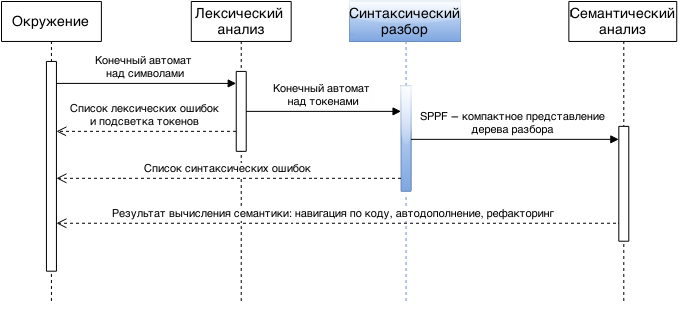
\includegraphics[width=15cm]{pictures/Seq_YC.png}
 \caption{Диаграмма последовательности: взаимодействие компонентов
инструмента YaccConstructor (рисунок взят из работы~\cite{EkaterinaMaster})}
 \label{seq}
\end{figure}